% Options for packages loaded elsewhere
\PassOptionsToPackage{unicode}{hyperref}
\PassOptionsToPackage{hyphens}{url}
\PassOptionsToPackage{dvipsnames,svgnames,x11names}{xcolor}
%
\documentclass[
  twocolumn]{article}

\usepackage{amsmath,amssymb}
\usepackage{iftex}
\ifPDFTeX
  \usepackage[T1]{fontenc}
  \usepackage[utf8]{inputenc}
  \usepackage{textcomp} % provide euro and other symbols
\else % if luatex or xetex
  \usepackage{unicode-math}
  \defaultfontfeatures{Scale=MatchLowercase}
  \defaultfontfeatures[\rmfamily]{Ligatures=TeX,Scale=1}
\fi
\usepackage{lmodern}
\ifPDFTeX\else  
    % xetex/luatex font selection
\fi
% Use upquote if available, for straight quotes in verbatim environments
\IfFileExists{upquote.sty}{\usepackage{upquote}}{}
\IfFileExists{microtype.sty}{% use microtype if available
  \usepackage[]{microtype}
  \UseMicrotypeSet[protrusion]{basicmath} % disable protrusion for tt fonts
}{}
\makeatletter
\@ifundefined{KOMAClassName}{% if non-KOMA class
  \IfFileExists{parskip.sty}{%
    \usepackage{parskip}
  }{% else
    \setlength{\parindent}{0pt}
    \setlength{\parskip}{6pt plus 2pt minus 1pt}}
}{% if KOMA class
  \KOMAoptions{parskip=half}}
\makeatother
\usepackage{xcolor}
\setlength{\emergencystretch}{3em} % prevent overfull lines
\setcounter{secnumdepth}{-\maxdimen} % remove section numbering
% Make \paragraph and \subparagraph free-standing
\ifx\paragraph\undefined\else
  \let\oldparagraph\paragraph
  \renewcommand{\paragraph}[1]{\oldparagraph{#1}\mbox{}}
\fi
\ifx\subparagraph\undefined\else
  \let\oldsubparagraph\subparagraph
  \renewcommand{\subparagraph}[1]{\oldsubparagraph{#1}\mbox{}}
\fi


\providecommand{\tightlist}{%
  \setlength{\itemsep}{0pt}\setlength{\parskip}{0pt}}\usepackage{longtable,booktabs,array}
\usepackage{calc} % for calculating minipage widths
% Correct order of tables after \paragraph or \subparagraph
\usepackage{etoolbox}
\makeatletter
\patchcmd\longtable{\par}{\if@noskipsec\mbox{}\fi\par}{}{}
\makeatother
% Allow footnotes in longtable head/foot
\IfFileExists{footnotehyper.sty}{\usepackage{footnotehyper}}{\usepackage{footnote}}
\makesavenoteenv{longtable}
\usepackage{graphicx}
\makeatletter
\def\maxwidth{\ifdim\Gin@nat@width>\linewidth\linewidth\else\Gin@nat@width\fi}
\def\maxheight{\ifdim\Gin@nat@height>\textheight\textheight\else\Gin@nat@height\fi}
\makeatother
% Scale images if necessary, so that they will not overflow the page
% margins by default, and it is still possible to overwrite the defaults
% using explicit options in \includegraphics[width, height, ...]{}
\setkeys{Gin}{width=\maxwidth,height=\maxheight,keepaspectratio}
% Set default figure placement to htbp
\makeatletter
\def\fps@figure{htbp}
\makeatother
% definitions for citeproc citations
\NewDocumentCommand\citeproctext{}{}
\NewDocumentCommand\citeproc{mm}{%
  \begingroup\def\citeproctext{#2}\cite{#1}\endgroup}
\makeatletter
 % allow citations to break across lines
 \let\@cite@ofmt\@firstofone
 % avoid brackets around text for \cite:
 \def\@biblabel#1{}
 \def\@cite#1#2{{#1\if@tempswa , #2\fi}}
\makeatother
\newlength{\cslhangindent}
\setlength{\cslhangindent}{1.5em}
\newlength{\csllabelwidth}
\setlength{\csllabelwidth}{3em}
\newenvironment{CSLReferences}[2] % #1 hanging-indent, #2 entry-spacing
 {\begin{list}{}{%
  \setlength{\itemindent}{0pt}
  \setlength{\leftmargin}{0pt}
  \setlength{\parsep}{0pt}
  % turn on hanging indent if param 1 is 1
  \ifodd #1
   \setlength{\leftmargin}{\cslhangindent}
   \setlength{\itemindent}{-1\cslhangindent}
  \fi
  % set entry spacing
  \setlength{\itemsep}{#2\baselineskip}}}
 {\end{list}}
\usepackage{calc}
\newcommand{\CSLBlock}[1]{\hfill\break\parbox[t]{\linewidth}{\strut\ignorespaces#1\strut}}
\newcommand{\CSLLeftMargin}[1]{\parbox[t]{\csllabelwidth}{\strut#1\strut}}
\newcommand{\CSLRightInline}[1]{\parbox[t]{\linewidth - \csllabelwidth}{\strut#1\strut}}
\newcommand{\CSLIndent}[1]{\hspace{\cslhangindent}#1}

% load packages
\usepackage{geometry}
\usepackage{xcolor}
\usepackage{eso-pic}

%% Set page size with a wider right margin
\geometry{a4paper, left=10mm, top=10mm, bottom=10mm, right=10mm}


%% Let's define some colours
\definecolor{RSSyellow}{HTML}{d3a435}
\definecolor{RSSblue}{HTML}{005573}

%% Let's add a logo to the upper right
% \AddToShipoutPicture{% 
%      % logo
%     \AtPageUpperLeft{% start the bar at the bottom right of the page
%         \put(\LenToUnit{\dimexpr\paperwidth-2.25cm},27.2cm){% move it to the top right
%             \color{white}
\includegraphics[width=2cm]{images/cdc.png}
%           }%
%      }%
% }

\newcommand\UpperLeftImage{%
     \put(10,\LenToUnit{\dimexpr\paperwidth + 50mm}){%
          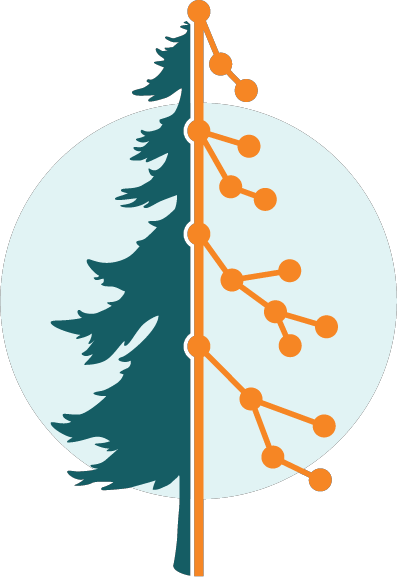
\includegraphics[width=2cm,height=2cm]{images/nwpage_tree_logo.png}%
     }%
}

\newcommand\UpperRightImage{%
     \put(180mm,\LenToUnit{\dimexpr\paperwidth + 50mm}){%
          
\includegraphics[width=2cm,height=2cm]{images/cdc.png}%
     }%
}

% Add images to every page
\AddToShipoutPictureBG{%
     \UpperLeftImage%
     \UpperRightImage%
}
\makeatletter
\@ifpackageloaded{caption}{}{\usepackage{caption}}
\AtBeginDocument{%
\ifdefined\contentsname
  \renewcommand*\contentsname{Table of contents}
\else
  \newcommand\contentsname{Table of contents}
\fi
\ifdefined\listfigurename
  \renewcommand*\listfigurename{List of Figures}
\else
  \newcommand\listfigurename{List of Figures}
\fi
\ifdefined\listtablename
  \renewcommand*\listtablename{List of Tables}
\else
  \newcommand\listtablename{List of Tables}
\fi
\ifdefined\figurename
  \renewcommand*\figurename{Figure}
\else
  \newcommand\figurename{Figure}
\fi
\ifdefined\tablename
  \renewcommand*\tablename{Table}
\else
  \newcommand\tablename{Table}
\fi
}
\@ifpackageloaded{float}{}{\usepackage{float}}
\floatstyle{ruled}
\@ifundefined{c@chapter}{\newfloat{codelisting}{h}{lop}}{\newfloat{codelisting}{h}{lop}[chapter]}
\floatname{codelisting}{Listing}
\newcommand*\listoflistings{\listof{codelisting}{List of Listings}}
\makeatother
\makeatletter
\makeatother
\makeatletter
\@ifpackageloaded{caption}{}{\usepackage{caption}}
\@ifpackageloaded{subcaption}{}{\usepackage{subcaption}}
\makeatother
\ifLuaTeX
  \usepackage{selnolig}  % disable illegal ligatures
\fi
\usepackage{bookmark}

\IfFileExists{xurl.sty}{\usepackage{xurl}}{} % add URL line breaks if available
\urlstyle{same} % disable monospaced font for URLs
\hypersetup{
  pdftitle={Pathogen Genomics Center of Excellence Situation Report},
  colorlinks=true,
  linkcolor={RSSblue},
  filecolor={Maroon},
  citecolor={Blue},
  urlcolor={RSSblue},
  pdfcreator={LaTeX via pandoc}}

\title{Pathogen Genomics Center of Excellence Situation Report}
\author{}
\date{2024-04-26}

\begin{document}
\maketitle

\section{Key Findings}\label{key-findings}

\begin{itemize}
\tightlist
\item
  Current data reflects a mixture of JN.1 descendents as the likely near
  term variants.\\
\item
  Globally no other variants with unusual characteristics have been
  identified as having unusual growth.
\item
  Some other point
\end{itemize}

\section{Situation Update Details}\label{situation-update-details}

\begin{itemize}
\tightlist
\item
  Based on what - XYZ(?), JN.1 and descendents continue to dominate.
  Some recombinations from JN.1 and other BA.5 variants are being
  monitoredtracked, but have yet to show significant growth relative
  other variants.
\item
  Together this diversity suggests steady evolution against general
  population immunity with no indications of a variant driven wave of
  COVID-19 infections.
\item
  As of MM/DD/YYYY, there were X samples from MM/DD/YYYY - MM/DD/YYYY,
  some comment on trend
\item
  Some text here about image one. There is this variant that's here
\item
  Some text about image two
\item
  Image 3 has this
\item
  Findings from a site's analysis of national data
\end{itemize}

\begin{figure}[H]

\centering{

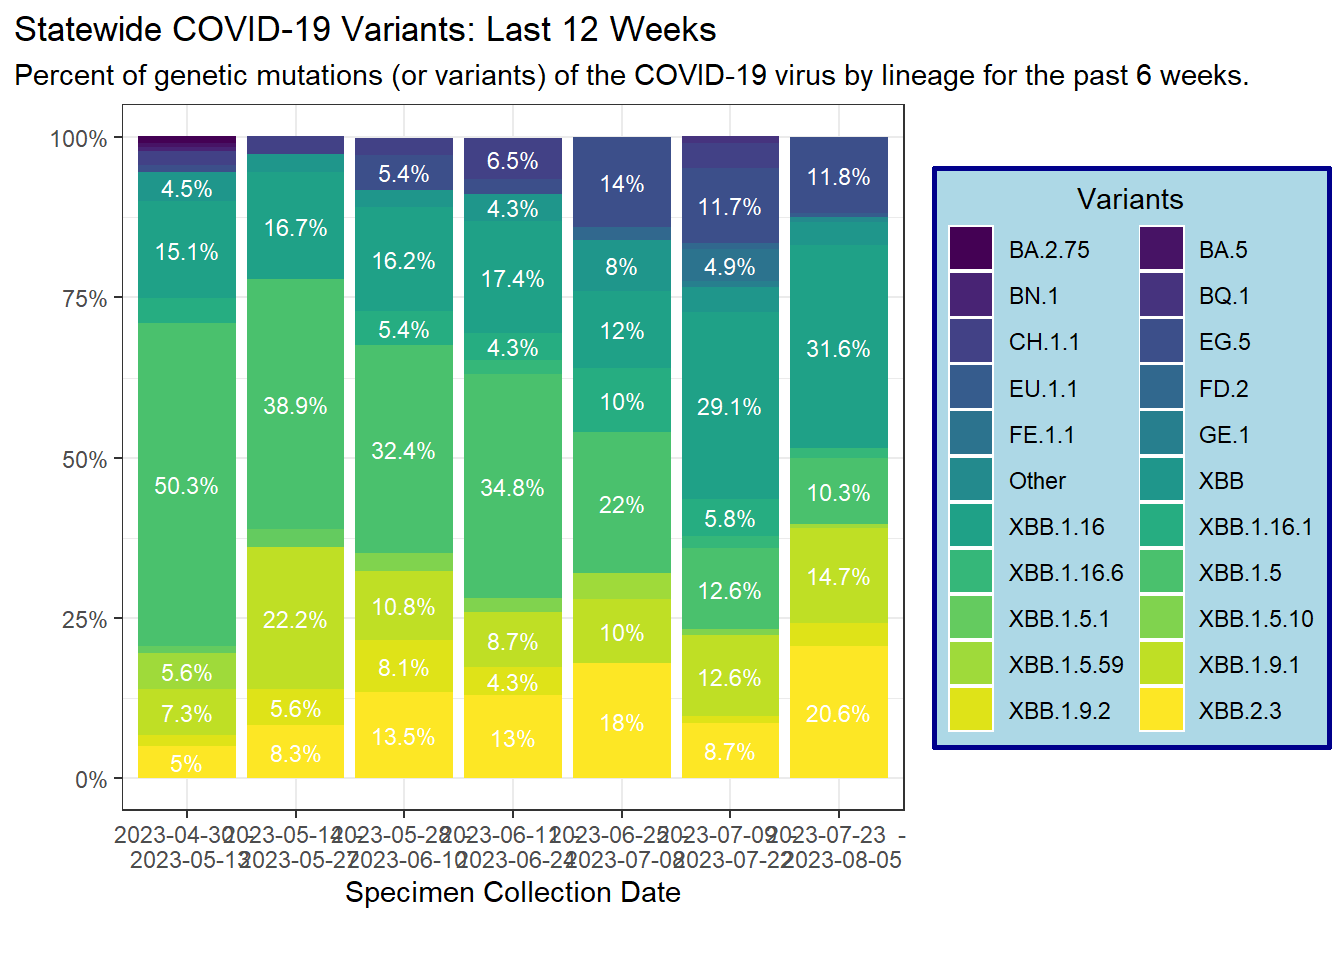
\includegraphics{index_files/figure-latex/notebooks-nwcoe-fig-countprop-output-1.png}

}

\caption{\label{fig-countprop}Proportion of variants by year.}

\end{figure}%

\textsubscript{Source:
\href{https://coe-test-org.github.io/sitrep-demo/notebooks/nwcoe-preview.html\#cell-fig-countprop}{NorthWest
Genomics Center of Excellence}}

\begin{figure}[H]

\centering{

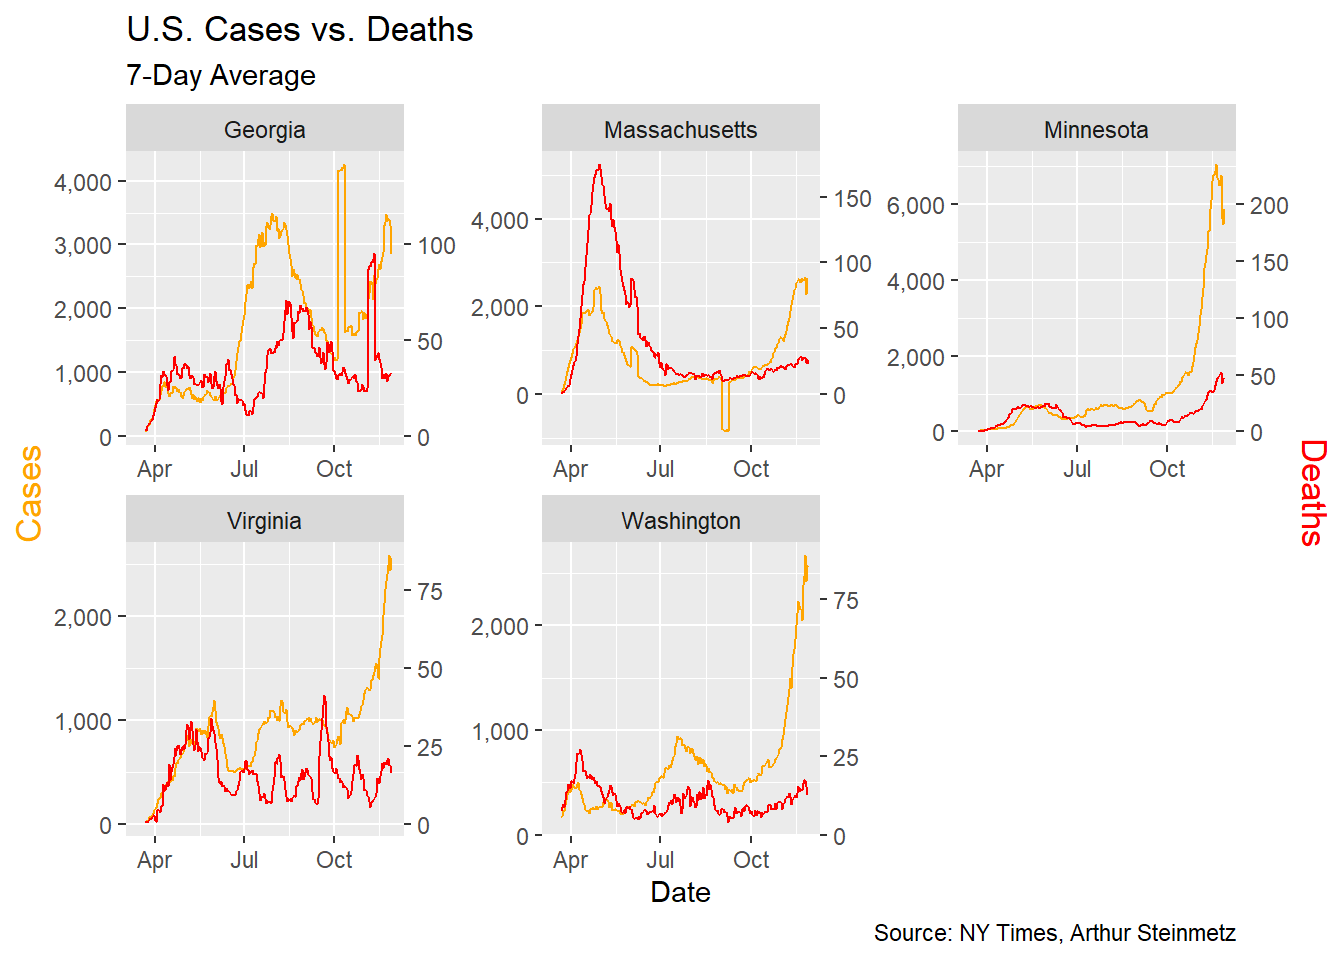
\includegraphics{index_files/figure-latex/notebooks-necoe-fig-state-analysis-output-2.png}

}

\caption{\label{fig-state-analysis}From the New York Times: A couple of
observations are obvious. First when cases start to rise, deaths follow
with a lag. Second, we have had three spikes in cases so far and in each
successive instance the mortality has risen by a smaller amount. This
suggests that, thankfully, we are getting better at treating this
disease. It is NOT a function of increased testing because positivity
rates have not been falling.}

\end{figure}%

\textsubscript{Source:
\href{https://coe-test-org.github.io/sitrep-demo/notebooks/necoe-preview.html\#cell-fig-state-analysis}{New
England Genomics Center of Excellence}}

\begin{figure}[H]

\centering{

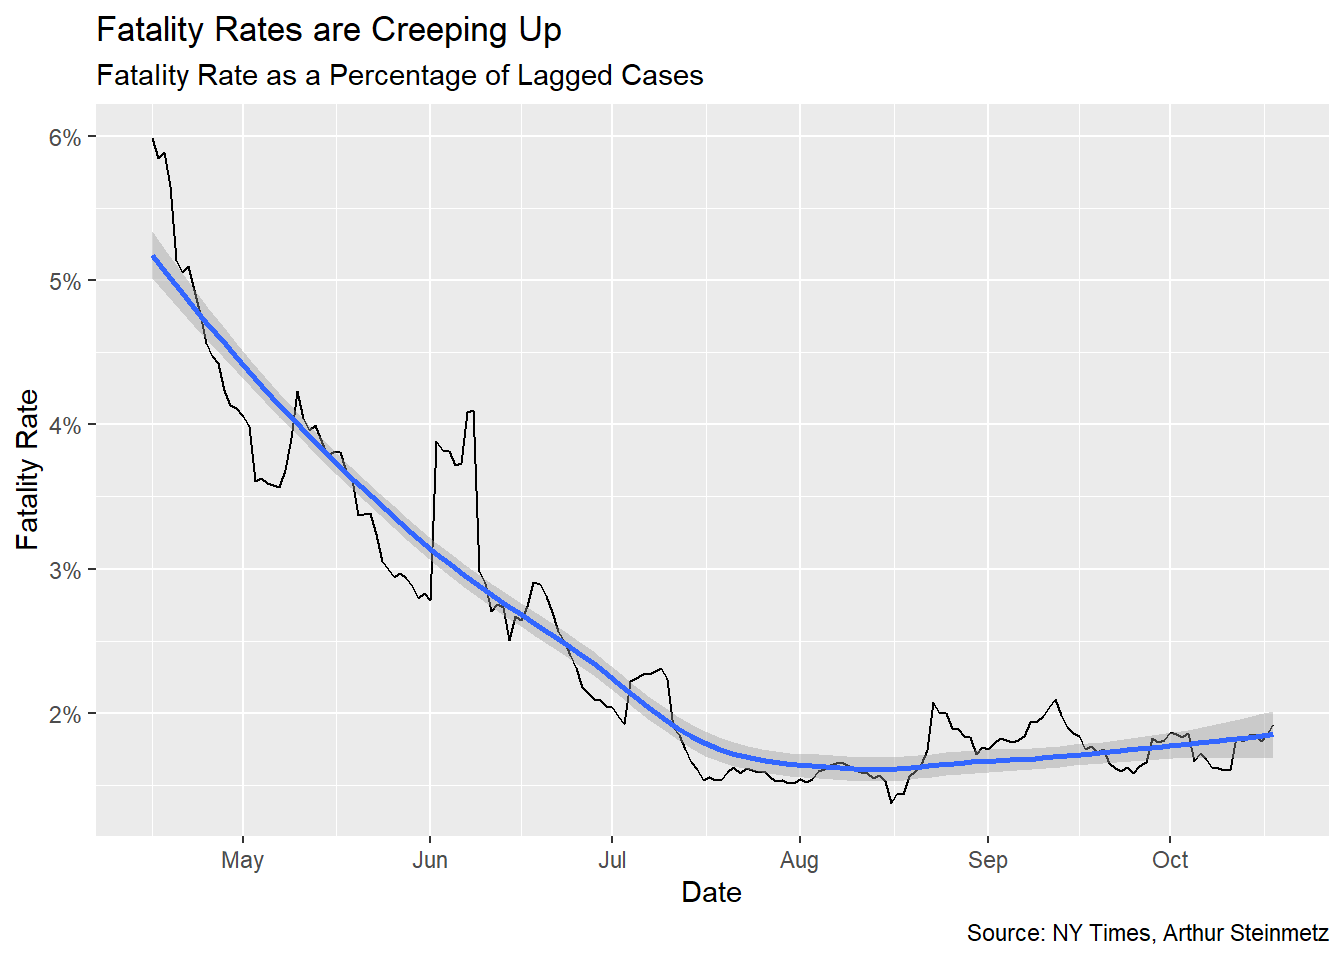
\includegraphics{index_files/figure-latex/notebooks-vacoe-fig-fatality-plot-output-2.png}

}

\caption{\label{fig-fatality-plot}COVID-19 fatalities, outputs from New
York Times modeling.}

\end{figure}%

\textsubscript{Source:
\href{https://coe-test-org.github.io/sitrep-demo/notebooks/vacoe-preview.html\#cell-fig-fatality-plot}{Virginia
Genomics Center of Excellence}}

\section{Site Summaries}\label{site-summaries}

\textsubscript{Source:
\href{https://coe-test-org.github.io/sitrep-demo/index.qmd.html}{Article
Notebook}}

\begin{itemize}
\tightlist
\item
  Washington State Department of Health - highest variant proportion is
  50\%
\item
  Georgia Department of Public Health probablity of detection: 60 and
  the consensus genomes are uploaded to public repositories like GISAID
  and GenBank.
\item
  Massachusetts Department of Health prop - 50
\item
  Virginia Deparment of Health - 60\%
\end{itemize}

\subsection{Section}\label{section}

This is a simple placeholder for the manuscript's main document (Knuth
1984).

\begin{itemize}
\tightlist
\item
  To monitor SARS-CoV-2 in Washington state, Washington state Department
  of Health (WA DOH) implemented a Sentinel Surveillance system, a type
  of genomic surveillance that tracks SARS-CoV-2 variants across the
  state.
\item
  Laboratories across the state, including the Washington state Public
  Health Laboratories (PHL) will sequence SARS-CoV-2 from collected
  specimens. Raw sequencing data is assembled into consensus genomes
  using publicly available bioinformatics pipeline, and the consensus
  genomes are uploaded to public repositories like GISAID and GenBank.
  This report demonstrates how the NW PGCoE utilizes SARS-CoV-2
  sequencing data to monitor emerging variants biweekly, forecast
  emerging SARS-CoV-2 variants, and infers relative abundance estimates
  of SARS-CoV-2 variants in the wastewater. Previous work that looked at
  the disease severity of SARS-CoV-2 variants is currently being
  implemented to analyze the disease severity of current variants
  utilizing hospitalization data. This work is ongoing and will be
  presented at a later time.
\end{itemize}

\phantomsection\label{refs}
\begin{CSLReferences}{1}{0}
\bibitem[\citeproctext]{ref-knuth84}
Knuth, Donald E. 1984. {``Literate Programming.''} \emph{Comput. J.} 27
(2): 97--111. \url{https://doi.org/10.1093/comjnl/27.2.97}.

\end{CSLReferences}



\end{document}
